\documentclass[tikz,border=4pt]{standalone}
% Paleta y fuentes compartidas por el libro y las figuras (única fuente de verdad).
\RequirePackage{xcolor}
\definecolor{oxido}{HTML}{B7410E}
\definecolor{cobre}{HTML}{D27D2D}
\definecolor{carbon}{HTML}{2B2B2B}
\definecolor{azul}{HTML}{1F5F8B}
\definecolor{arena}{HTML}{F4EDE4}

\usepackage{fontspec}
\setsansfont{FiraSans}[Extension=.otf,UprightFont=*-Regular,BoldFont=*-Bold,ItalicFont=*-Italic,BoldItalicFont=*-BoldItalic]
\setmonofont{FiraMono}[Extension=.otf,UprightFont=*-Regular,BoldFont=*-Medium]
\usetikzlibrary{positioning,arrows.meta,calc}
\begin{document}
\sffamily\small
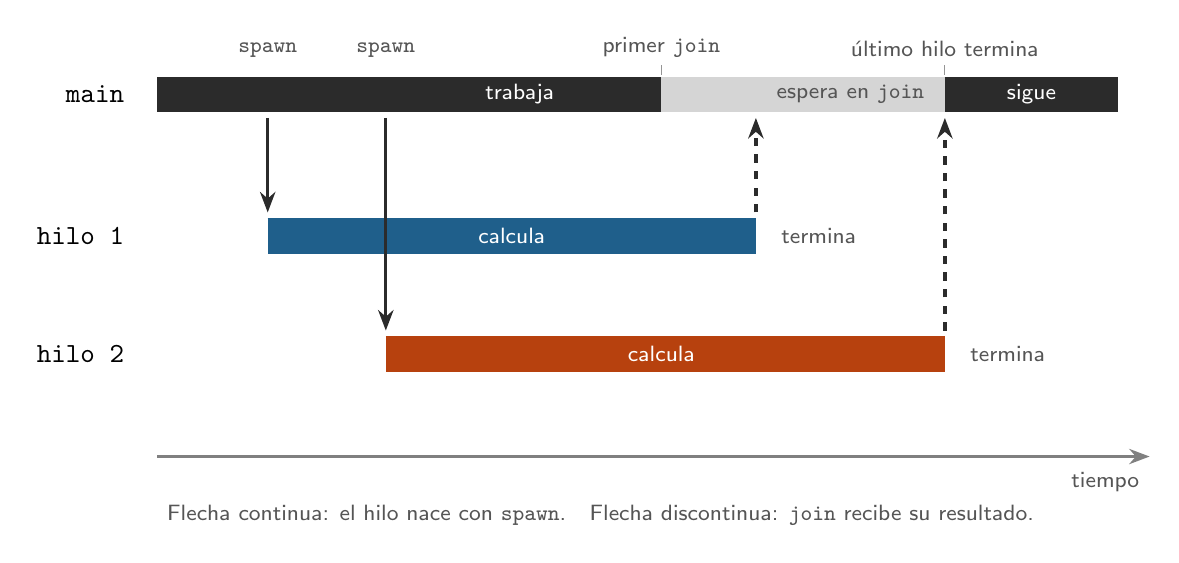
\begin{tikzpicture}[>={Stealth[length=2.6mm]},
  carril/.style={font=\ttfamily\bfseries,anchor=east},
  nota/.style={font=\sffamily\footnotesize,text=carbon!80,align=center},
  barra/.style={line width=4.5mm}]
  % Carriles: main arriba, dos hilos debajo
  \node[carril] at (-0.3,0) {main};
  \node[carril] at (-0.3,-1.8) {hilo 1};
  \node[carril] at (-0.3,-3.3) {hilo 2};
  % Eje de tiempo
  \draw[->,thick,carbon!60] (0,-4.6) -- (12.6,-4.6)
    node[anchor=north east,nota,yshift=-2pt] {tiempo};
  % main: trabaja, espera en join, sigue
  \draw[barra,carbon] (0,0) -- (6.4,0);
  \draw[barra,carbon!20] (6.4,0) -- (10.0,0);
  \draw[barra,carbon] (10.0,0) -- (12.2,0);
  \node[nota,text=white] at (4.6,0) {trabaja};
  \node[nota] at (8.8,0) {espera en \texttt{join}};
  \node[nota,text=white] at (11.1,0) {sigue};
  % hilos lanzados
  \draw[barra,azul] (1.4,-1.8) -- (7.6,-1.8);
  \draw[barra,oxido] (2.9,-3.3) -- (10.0,-3.3);
  \node[nota,text=white] at (4.5,-1.8) {calcula};
  \node[nota,text=white] at (6.4,-3.3) {calcula};
  % spawn
  \draw[->,very thick,carbon] (1.4,-0.3) -- (1.4,-1.5);
  \draw[->,very thick,carbon] (2.9,-0.3) -- (2.9,-3.0);
  \node[nota,anchor=south] at (1.4,0.35) {\texttt{spawn}};
  \node[nota,anchor=south] at (2.9,0.35) {\texttt{spawn}};
  % join
  \draw[->,very thick,carbon,dashed] (7.6,-1.5) -- (7.6,-0.3);
  \draw[->,very thick,carbon,dashed] (10.0,-3.0) -- (10.0,-0.3);
  \node[nota,anchor=south] at (6.4,0.35) {primer \texttt{join}};
  \draw[carbon!50] (6.4,0.25) -- (6.4,0.37);
  \node[nota,anchor=south] at (10.0,0.35) {último hilo termina};
  \draw[carbon!50] (10.0,0.25) -- (10.0,0.37);
  % notas de resultados
  \node[nota,anchor=west] at (7.8,-1.8) {termina};
  \node[nota,anchor=west] at (10.2,-3.3) {termina};
  % leyenda
  \node[nota,anchor=west] at (0,-5.35) {Flecha continua: el hilo nace con \texttt{spawn}.\quad
    Flecha discontinua: \texttt{join} recibe su resultado.};
\end{tikzpicture}
\end{document}
